\section{How Many Developers Can Share One Server?}\label{sec:agent}

Measured by monthly output, one pod covers \dv{agent.E13.agent.seats_volume_u100} developers of the usage profile we
observed at full utilization and \dv{agent.E13.agent.seats_volume_u50} at half. Measured by how many can see the model
write at 40 tokens/s or more at the same moment, it covers about \dv{agent.E13.agent.seats_conc_e1}, and that is the
number to plan with. The pod is the bar of the introduction, able to pour for a whole office every night but with four
stools at the counter. When more than four regulars want a drink at once, everyone is served more slowly, so the
number of stools decides how many regulars the bar can take. This section measures the stools and counts the
regulars.

The comparison is about serving capacity and infrastructure cost. It does not claim that DeepSeek-V4.1-Flash is
equivalent in quality or capability to the models behind a commercial coding agent. A subscription such as Claude
Code buys a complete product (the agent, its tools, model access, reliability and support), while the self-hosted
figures below are GPU rental only unless stated otherwise.

\paragraph{What a developer consumes.}
We started from one developer's Claude Code usage screen for seven days (\datafile{experiments/agent_workload.yaml}).
It reports \dv{agent.sample.total_week} tokens over \dv{agent.sample.sessions} sessions on
\dv{agent.sample.active_days} active days. Of those, the model wrote \dv{agent.sample.output_week}, or
\dv{agent.sample.output_share_pct}\%. Another \dv{agent.sample.cache_read_week} were cached context read again,
\dv{agent.sample.cache_write_week} were new context written to the cache and \dv{agent.sample.input_week} were
uncached input. A coding agent mostly re-reads. Per token it writes, this profile reads
\dv{agent.ratio.read_per_output} tokens of cached context and adds \dv{agent.ratio.write_per_output} new ones. With
replies of \dv{agent.turn.output} tokens (our assumption), a turn reads about \dv{agent.turn.context_read} tokens of
context and adds about \dv{agent.turn.new_tokens}. These are the provider's billing categories, not vLLM's accounting
of its prefix cache, so the profile shapes our synthetic workload without claiming token-for-token equivalence. One
developer of this profile receives \dv{agent.dev.output_month} million output tokens a month.

\paragraph{Two capacities.}
The two answers differ because two capacities are at work. The \emph{simultaneous-stream capacity} $C$ is the largest
number of streams for which that level and every smaller one keep a median rate per stream of at least 40 tokens/s
(25\,ms per token) and stay within the harness's error rule. Total throughput never counts as success here, since ten
streams at 20 tokens/s are not five at 40. The \emph{volume capacity} divides the output a pod produces in a month, at
the total rate measured at $C$ and a stated utilization, by one developer's monthly output. In the bar picture, $C$ is
the number of stools and the volume capacity is how much the bar can pour.

\paragraph{Four stools.}
Every context regime we ran to four streams keeps at least 40 tokens/s per stream up to four and loses it between
five and eight (Figure~\ref{fig:agent}, Table~\ref{tab:agent-capacity}). Independent 256K-token contexts were run only
up to three streams, all above the objective. We provision with a 10\% margin (44 tokens/s), because levels measured
once and within a few tokens/s of 40 pass or fail by noise. The shared 128K prefix passed at five and the agent turns
at six by less than one token/s each, and the shared 256K prefix failed at five just below the line and passed at six.
With the margin the capacity is \dv{agent.E13.short.Cprov} for short sessions, \dv{agent.E13.cached128k.Cprov} and
\dv{agent.E13.cached256k.Cprov} for shared 128K and 256K prefixes, \dv{agent.E13.own128k.Cprov} for independent 128K
contexts, \dv{agent.E13.own256k.Cprov_text} for independent 256K contexts and \dv{agent.E13.agent.Cprov} for agent
turns. At four agent-turn streams each one gets a median of \dv{agent.E13.agent.prov.rate_p50} tokens/s (p5
\dv{agent.E13.agent.prov.rate_p5}), TTFT p95 is \dv{agent.E13.agent.prov.ttft_p95}\,s and the pod writes
\dv{agent.E13.agent.prov.agg} tokens/s in total. At eight streams the median falls to
\dv{agent.E13.agent.fail.rate_p50}.

These capacities come from experiment E13 (\datafile{experiments/workloads/agent.yaml}, runner
\datafile{experiments/runs/agent.sh}), one boot of the \texttt{gen30} stack in \dv{lean.session3.minutes} minutes with
400-token replies. Its regimes cover how coding agents use context, and the tables use their names. In
\emph{short} sessions each stream has a unique 4K-token prompt. With a \emph{shared prefix} all streams branch from one
cached prefix of 128K or 256K tokens, like several agents on the same codebase. With an \emph{own context} each stream
owns an independent cached context of 128K or 256K tokens, extended by 512 new tokens per turn. \emph{Agent turns}
follow the observed ratios, each stream owning a context of 88,000 tokens that grows by 3,500 tokens per turn. In the
short and shared-prefix regimes the number of streams grew through 1, 2, 3, 4, 5, 6, 8 and 12 and stopped after two
levels below the objective, while the own-context regimes and agent turns ran fixed lists because of KV-cache and time
limits (own 128K up to five, own 256K up to three, agent turns at 1, 2, 3, 4, 6 and 8). The rate per stream is the reply's tokens over the
time from its first token to the end of the stream, which stays valid for the \dv{agent.E13.all.bursts} of
\dv{agent.E13.all.requests} requests whose reply arrived mostly in one late chunk. No request failed.

The length of the context barely matters once it is cached. The 256K-token regimes are no slower than the short one at
the same number of streams, because the time to write is dominated by the size of the batch, not by attention over the
cached context. Memory was not the limit either. Five independent 128K contexts and three of 256K ran with at most
\dv{agent.E13.own.kv_max_pct}\% of the KV cache in use (the session's maximum, \dv{agent.E13.all.kv_max_pct}\%, came
from eight agent-turn streams), and no request was paused to free memory (\dv{agent.E13.all.preemptions}
preemptions). vLLM's own estimate was \dv{ctl.kv.max_concurrency} full-length requests, so for this model's compressed
attention it is conservative. GPU memory stayed between \dv{agent.E13.all.gpu_mem_min} and
\dv{agent.E13.all.gpu_mem_max}\,GiB per GPU, host memory peaked at \dv{agent.E13.all.host_max}\,GiB, and PCIe reads
grew with load (Table~\ref{tab:agent-resources}).

\begin{figure}[t]
\centering
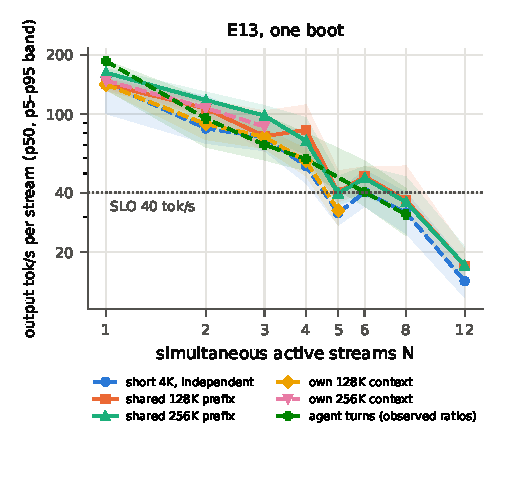
\includegraphics[width=0.49\linewidth]{figures/generated/agent_stream_rate.pdf}\hfill
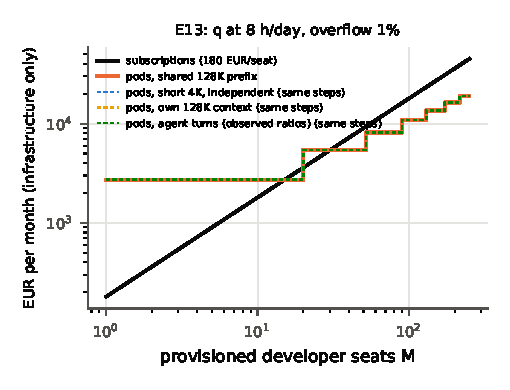
\includegraphics[width=0.49\linewidth]{figures/generated/agent_cost_seats.pdf}
\caption{Coding-agent case study, E13 (one boot). Left: median output rate per stream against simultaneous streams
(bands: p5 to p95 of requests), with the 40 tokens/s objective. Dashed lines are independent contexts. Right: monthly
cost of subscriptions and of the pods needed for $M$ provisioned seats, the larger of the volume and the concurrency
requirement (capacity with a 10\% margin, 50\% utilization, duty cycle for an 8-hour window, overflow probability 1\%),
infrastructure only. The four pod curves coincide because every regime has the same provisioning capacity.}
\label{fig:agent}
\end{figure}

% Generated by hostoffload.analysis.pipeline. Do not edit.
\begin{table}[t]
\centering
\small
\begin{fittable}{tab:agent-capacity}
\begin{tabular}{llrrrrrrrr}
\toprule
regime & source & C & C$_{+10\%}$ & p5 & p50 & p95 & TTFT p95 & aggr. & fails at \\
\midrule
short 4K, independent & E13 & 4 & 4 & 45 & 55 & 80 & 1.15 & 131 & 5 (32) \\
shared 128K prefix & E13 & 6 & 4 & 40 & 48 & 54 & 0.87 & 176 & 8 (37) \\
shared 256K prefix & E13 & 4 & 4 & 62 & 73 & 96 & 1.30 & 155 & 5 (40) \\
own 128K context & E13 & 4 & 4 & 49 & 58 & 67 & 1.72 & 172 & 5 (32) \\
own 256K context & E13 & $\ge$3 & $\ge$3 & 65 & 87 & 95 & 1.76 & 155 & - \\
agent turns (observed ratios) & E13 & 6 & 4 & 34 & 40 & 58 & 2.99 & 178 & 8 (31) \\
\bottomrule
\end{tabular}
\end{fittable}
\caption{Simultaneous streams at a median of at least 40 output tokens/s per stream. C is the largest N whose level and every smaller tested level meet it (failing on 2 or more errors above 5\%); per-stream rates (p5, p50, p95, tokens/s) and TTFT p95 (s) at C; the last column is the first failing N with its median rate. C$_{+10\%}$ is the same with a 10\% margin (44 tokens/s), used for provisioning.}
\label{tab:agent-capacity}
\end{table}

% Generated by hostoffload.analysis.pipeline. Do not edit.
\begin{table}[t]
\centering
\small
\begin{fittable}{tab:agent-levels}
\begin{tabular}{lrrrrrrrrrr}
\toprule
regime & N & rate p5 & p50 & p95 & TPOT p50 & p95 & TTFT p50 & p95 & err \% & aggr. \\
\midrule
short & 1 & 101 & 144 & 156 & 7.0 & 10.1 & 0.66 & 18.22 & 0 & 38 \\
short & 2 & 71 & 85 & 124 & 11.9 & 14.1 & 0.68 & 1.03 & 0 & 84 \\
short & 3 & 65 & 77 & 93 & 13.1 & 15.3 & 0.72 & 0.82 & 0 & 115 \\
short & 4 & 45 & 55 & 80 & 18.5 & 22.4 & 0.73 & 1.15 & 0 & 131 \\
short & 5 & 27 & 32 & 41 & 31.7 & 36.6 & 0.85 & 1.39 & 0 & 110 \\
short & 6 & 34 & 40 & 52 & 24.9 & 29.4 & 0.85 & 1.38 & 0 & 157 \\
short & 8 & 25 & 32 & 40 & 31.6 & 40.2 & 0.90 & 1.65 & 0 & 147 \\
short & 12 & 12 & 14 & 18 & 70.2 & 85.0 & 1.53 & 2.61 & 0 & 120 \\
cached128k & 1 & 132 & 142 & 152 & 7.0 & 7.6 & 0.61 & 0.63 & 0 & 118 \\
cached128k & 2 & 98 & 107 & 119 & 9.3 & 10.2 & 0.62 & 0.68 & 0 & 141 \\
cached128k & 3 & 69 & 77 & 104 & 12.9 & 14.6 & 0.72 & 0.80 & 0 & 145 \\
cached128k & 4 & 58 & 83 & 112 & 12.1 & 17.3 & 0.64 & 0.84 & 0 & 135 \\
cached128k & 5 & 36 & 40 & 52 & 25.0 & 27.8 & 0.74 & 0.88 & 0 & 155 \\
cached128k & 6 & 40 & 48 & 54 & 20.7 & 24.8 & 0.79 & 0.87 & 0 & 176 \\
cached128k & 8 & 32 & 37 & 55 & 27.3 & 31.8 & 0.84 & 1.00 & 0 & 178 \\
cached128k & 12 & 14 & 17 & 21 & 58.8 & 72.3 & 1.04 & 1.50 & 0 & 146 \\
cached256k & 1 & 146 & 162 & 171 & 6.2 & 6.8 & 0.96 & 1.02 & 0 & 113 \\
cached256k & 2 & 114 & 118 & 129 & 8.5 & 8.8 & 0.99 & 1.00 & 0 & 128 \\
cached256k & 3 & 77 & 98 & 111 & 10.2 & 13.1 & 1.02 & 1.17 & 0 & 155 \\
cached256k & 4 & 62 & 73 & 96 & 13.7 & 16.0 & 1.04 & 1.30 & 0 & 155 \\
cached256k & 5 & 35 & 40 & 48 & 25.2 & 28.8 & 1.08 & 1.53 & 0 & 131 \\
cached256k & 6 & 38 & 47 & 54 & 21.1 & 26.0 & 1.09 & 1.34 & 0 & 166 \\
cached256k & 8 & 32 & 36 & 48 & 27.9 & 31.7 & 1.34 & 1.67 & 0 & 212 \\
cached256k & 12 & 14 & 17 & 21 & 58.5 & 70.5 & 1.31 & 1.57 & 0 & 132 \\
own128k & 1 & 132 & 141 & 151 & 7.1 & 7.6 & 0.78 & 0.82 & 0 & 103 \\
own128k & 2 & 74 & 89 & 103 & 5.7 & 13.0 & 0.76 & 1.12 & 0 & 121 \\
own128k & 3 & 67 & 77 & 84 & 13.0 & 15.0 & 0.93 & 1.37 & 0 & 174 \\
own128k & 4 & 49 & 58 & 67 & 17.2 & 20.5 & 0.94 & 1.72 & 0 & 172 \\
own128k & 5 & 27 & 32 & 40 & 27.3 & 35.6 & 1.00 & 2.07 & 0 & 120 \\
own256k & 1 & 135 & 148 & 161 & 3.1 & 5.9 & 1.05 & 1.06 & 0 & 99 \\
own256k & 2 & 100 & 108 & 118 & 9.3 & 10.0 & 1.06 & 1.39 & 0 & 147 \\
own256k & 3 & 65 & 87 & 95 & 11.6 & 15.7 & 1.23 & 1.76 & 0 & 155 \\
agent & 1 & 134 & 186 & 188 & 5.4 & 7.6 & 0.91 & 0.94 & 0 & 133 \\
agent & 2 & 68 & 95 & 119 & 9.8 & 14.8 & 0.91 & 1.47 & 0 & 123 \\
agent & 3 & 59 & 70 & 98 & 14.3 & 17.2 & 0.97 & 2.08 & 0 & 146 \\
agent & 4 & 52 & 59 & 80 & 16.9 & 19.5 & 1.24 & 2.34 & 0 & 168 \\
agent & 6 & 34 & 40 & 58 & 24.9 & 29.3 & 1.37 & 2.99 & 0 & 178 \\
agent & 8 & 24 & 31 & 42 & 31.7 & 41.3 & 1.57 & 4.22 & 0 & 186 \\
\bottomrule
\end{tabular}
\end{fittable}
\caption{Controlled: E13 per level, part 1 of 2, service per stream. Per-stream rate p5/p50/p95 (tokens/s, tokens over end of stream minus first token), TPOT p50/p95 (ms), TTFT p50/p95 (s), failed requests (\%) and aggregate output (tokens/s). Resources at the same levels: Table~\ref{tab:agent-resources}.}
\label{tab:agent-levels}
\end{table}
\begin{table}[t]
\centering
\small
\begin{fittable}{tab:agent-resources}
\begin{tabular}{lrrrrrrrr}
\toprule
regime & N & GPU GiB & host GiB & PCIe GB/s & KV \% & hit \% & preempt. & bursts \\
\midrule
short & 1 & 86.2 & 214 & 15.09 & 3 & 0 & 0 & 0 \\
short & 2 & 86.3 & 214 & 38.12 & 4 & 0 & 0 & 0 \\
short & 3 & 86.4 & 214 & 55.41 & 4 & 0 & 0 & 0 \\
short & 4 & 87.6 & 214 & 57.15 & 7 & 0 & 0 & 0 \\
short & 5 & 87.6 & 214 & 80.81 & 5 & 0 & 0 & 0 \\
short & 6 & 87.6 & 214 & 72.06 & 8 & 0 & 0 & 0 \\
short & 8 & 87.6 & 214 & 75.27 & 9 & 0 & 0 & 0 \\
short & 12 & 89.9 & 214 & 91.26 & 17 & 0 & 0 & 0 \\
cached128k & 1 & 90.0 & 214 & 26.47 & 10 & 100 & 0 & 0 \\
cached128k & 2 & 90.0 & 214 & 36.93 & 10 & 100 & 0 & 0 \\
cached128k & 3 & 90.0 & 214 & 52.07 & 10 & 100 & 0 & 0 \\
cached128k & 4 & 90.0 & 214 & 57.82 & 10 & 100 & 0 & 0 \\
cached128k & 5 & 90.0 & 214 & 78.94 & 10 & 100 & 0 & 0 \\
cached128k & 6 & 90.6 & 214 & 71.71 & 11 & 100 & 0 & 0 \\
cached128k & 8 & 90.0 & 214 & 78.56 & 11 & 100 & 0 & 0 \\
cached128k & 12 & 90.0 & 214 & 90.66 & 12 & 100 & 0 & 0 \\
cached256k & 1 & 90.1 & 214 & 27.92 & 19 & 100 & 0 & 0 \\
cached256k & 2 & 90.1 & 214 & 42.66 & 19 & 100 & 0 & 0 \\
cached256k & 3 & 90.1 & 214 & 50.80 & 19 & 100 & 0 & 0 \\
cached256k & 4 & 90.1 & 214 & 55.81 & 19 & 100 & 0 & 0 \\
cached256k & 5 & 90.1 & 214 & 75.80 & 19 & 100 & 0 & 0 \\
cached256k & 6 & 90.1 & 214 & 72.85 & 20 & 100 & 0 & 0 \\
cached256k & 8 & 90.1 & 214 & 76.37 & 20 & 100 & 0 & 0 \\
cached256k & 12 & 90.1 & 214 & 88.75 & 21 & 100 & 0 & 0 \\
own128k & 1 & 90.1 & 214 & 50.15 & 10 & 100 & 0 & 0 \\
own128k & 2 & 90.1 & 214 & 70.71 & 19 & 100 & 0 & 2 \\
own128k & 3 & 90.1 & 214 & 65.54 & 29 & 100 & 0 & 0 \\
own128k & 4 & 90.1 & 214 & 72.83 & 39 & 100 & 0 & 1 \\
own128k & 5 & 90.1 & 214 & 84.21 & 48 & 100 & 0 & 1 \\
own256k & 1 & 90.1 & 214 & 49.08 & 19 & 100 & 0 & 1 \\
own256k & 2 & 90.1 & 214 & 55.53 & 38 & 100 & 0 & 0 \\
own256k & 3 & 90.1 & 214 & 59.58 & 56 & 100 & 0 & 0 \\
agent & 1 & 90.1 & 214 & 48.96 & 7 & 96 & 0 & 0 \\
agent & 2 & 90.1 & 214 & 65.56 & 17 & 96 & 0 & 1 \\
agent & 3 & 90.1 & 214 & 64.25 & 25 & 96 & 0 & 0 \\
agent & 4 & 90.1 & 214 & 75.86 & 34 & 96 & 0 & 0 \\
agent & 6 & 90.1 & 214 & 77.57 & 53 & 96 & 0 & 0 \\
agent & 8 & 90.1 & 214 & 81.58 & 62 & 96 & 0 & 0 \\
\bottomrule
\end{tabular}
\end{fittable}
\caption{Controlled: E13 per level, part 2 of 2, resources. Peak GPU memory per GPU (GiB), peak host anon+shmem (GiB), mean PCIe RX summed over GPUs (GB/s), peak KV-cache use (\%), prefix-cache hit rate (\%), preemptions, and requests whose reply arrived in one late burst (their TPOT is invalid; the per-stream rate of Table~\ref{tab:agent-levels} stays valid).}
\label{tab:agent-resources}
\end{table}


\paragraph{From stools to regulars.}
Developers do not keep the model writing all day. Of a whole week, the model was busy for this developer about
\dv{agent.dev.busy_h_week} hours, \dv{agent.q.week}\% of the week. We count each output token at 40 tokens/s and each
new context token at the reading rate E12 measured for a 128K-token prompt (\dv{agent.prefill_tok_s} tokens/s), which
makes this an upper bound, since faster service shortens it. Spread over an 8-hour working window on each active day,
the chance that the developer needs a stream at a random moment of that window is $q=\dv{agent.q.h8}\%$
(\dv{agent.q.h4}\% for a 4-hour window, \dv{agent.q.h24}\% for 24).

If $M$ developers work independently with the same $q$, the number who need a stream at once follows approximately a
Binomial$(M,q)$ distribution. A pod with $C$ stools can take the largest $M$ for which more than $C$ need one at once
only rarely. For agent turns ($C=\dv{agent.E13.agent.Cprov}$) that is \dv{agent.E13.agent.seats_conc_e1} developers if
the overflow may happen in fewer than one moment in a hundred, and \dv{agent.E13.agent.seats_conc_e5} at five in a
hundred (Tables~\ref{tab:agent-seats} and~\ref{tab:agent-duty}). An overflow does not fail requests. It means that the
streams of that moment fall below 40 tokens/s. The model ignores correlation between developers (shared working
hours, deadlines) and bursts within a session, both of which make overflows more frequent, so these numbers are
optimistic for a team on one schedule.

By volume the same pod looks much larger. At the total rate measured at four agent-turn streams, its monthly output
equals \dv{agent.E13.agent.seats_volume_u100} developers of this profile at full utilization and
\dv{agent.E13.agent.seats_volume_u50} at 50\%. The pod has the volume for \dv{agent.E13.agent.volume_over_conc_u50} to
\dv{agent.E13.agent.volume_over_conc_u100} times more intermittent developers than it can serve at 40 tokens/s at the
same moment, so the stools set the limit (Figure~\ref{fig:two-capacities}).

\begin{figure}[t]
\centering
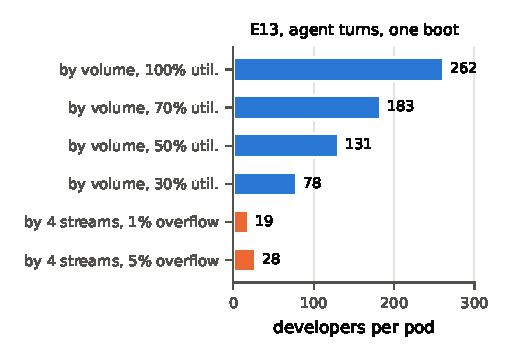
\includegraphics[width=0.62\linewidth]{figures/generated/agent_two_capacities.pdf}
\caption{The two capacities of one pod for agent turns (E13, one boot). Blue: developers whose monthly output the
pod can produce at the stated utilization. Orange: developers it can serve at 40 tokens/s or more each, with four
provisioned streams, an 8-hour active window and the stated probability that more than four want a stream at once.
Values from Table~\ref{tab:agent-seats}.}
\label{fig:two-capacities}
\end{figure}

To apply Table~\ref{tab:agent-duty} to another team, estimate how many hours a day its developers keep the agent
working, pick the row with that active window, and read the number of developers under the regime closest to how they
use context. A team that works in a narrower window concentrates its demand, so the same four stools take fewer
regulars.

% Generated by hostoffload.analysis.pipeline. Do not edit.
\begin{table}[t]
\centering
\small
\begin{fittable}{tab:agent-seats}
\begin{tabular}{lrrrrrrrrr}
\toprule
regime & C & aggr. & vol. 100\% & vol. 70\% & vol. 50\% & vol. 30\% & conc. 1\% & conc. 5\% & b.e. util. \% \\
\midrule
short 4K, independent & 4 & 131 & 204 & 143 & 102 & 61 & 19 & 28 & 7.4 \\
shared 128K prefix & 4 & 135 & 210 & 147 & 105 & 63 & 19 & 28 & 7.2 \\
shared 256K prefix & 4 & 155 & 242 & 169 & 121 & 73 & 19 & 28 & 6.3 \\
own 128K context & 4 & 172 & 268 & 188 & 134 & 81 & 19 & 28 & 5.6 \\
own 256K context & $\ge$3 & 155 & 242 & 170 & 121 & 73 & 12 & 20 & 6.2 \\
agent turns (observed ratios) & 4 & 168 & 262 & 183 & 131 & 78 & 19 & 28 & 5.8 \\
\bottomrule
\end{tabular}
\end{fittable}
\caption{Two capacities of one pod, provisioned on C with a 10\% margin (44 tokens/s). Volume: capacity-equivalent developer seats by observed monthly generation volume, at the aggregate output rate measured at that level and the stated utilization (these are NOT concurrent users). Concurrency: largest number of provisioned seats M with P(Binomial(M, q) > C) at most 1\% or 5\%, with q the duty cycle for an 8-hour active window. Last column: pod utilization at which the seats it serves would cost as much in subscriptions as the pod.}
\label{tab:agent-seats}
\end{table}

% Generated by hostoffload.analysis.pipeline. Do not edit.
\begin{table}[t]
\centering
\small
\begin{fittable}{tab:agent-duty}
\begin{tabular}{rrrrrrrr}
\toprule
active h/day & q \% & short & cached128k & cached256k & own128k & own256k & agent \\
\midrule
4 & 14.1 & 10 & 10 & 10 & 10 & 7 & 10 \\
8 & 7.1 & 19 & 19 & 19 & 19 & 12 & 19 \\
12 & 4.7 & 28 & 28 & 28 & 28 & 18 & 28 \\
24 & 2.4 & 55 & 55 & 55 & 55 & 36 & 55 \\
\bottomrule
\end{tabular}
\end{fittable}
\caption{Duty-cycle sensitivity. q is one developer's generating time (output at 40 tokens/s plus prefill of new tokens, from the usage sample) over an active window of the given hours on each of the 5 active days; cells are the largest M with P(Binomial(M, q) > C) at most 1\%.}
\label{tab:agent-duty}
\end{table}


\paragraph{What it costs against subscriptions.}
At \dv{agent.pod.eur_h}\,EUR an hour, a pod running all month costs \dv{agent.pod.eur_month}\,EUR, as much as
\dv{agent.break_even_seats} subscriptions of \dv{agent.seat_eur}\,EUR. One pod provisioned within its four stools
(\dv{agent.E13.agent.seats_conc_e1} developers) therefore lands just above break-even, and the next developer needs a
second pod, so 20 developers cost \dv{agent.E13.agent.cost.m20.extra}\,EUR a month more than subscriptions. Pooling
changes the picture, because the sum of many independent demands fluctuates less than each one. With load balanced
across pods, 100 developers need \dv{agent.E13.agent.cost.m100.pods} pods, \dv{agent.E13.agent.cost.m100.saving_pct}\%
below the cost of their subscriptions, and 250 need \dv{agent.E13.agent.cost.m250.pods},
\dv{agent.E13.agent.cost.m250.saving_pct}\% below, before engineering and operations (Table~\ref{tab:agent-cost},
Figure~\ref{fig:agent} right). Volume is never the constraint, since the pod breaks even at
\dv{agent.E13.agent.break_even_util}\% of its volume capacity. Stopping the pod outside a working window of
\dv{agent.pod.sched_hours} hours a month lowers its cost to \dv{agent.pod.sched_eur_month}\,EUR
(\dv{agent.break_even_seats_sched} subscriptions), but every start pays \dv{ctl.boot.min_minutes} to
\dv{ctl.boot.max_minutes} minutes of boot and weight loading and needs the \dv{static.pack.total_gib}\,GiB pack on
persistent storage. Engineering and operations move break-even substantially (Table~\ref{tab:agent-ops}), and those
amounts are assumptions, not measurements.

% Generated by hostoffload.analysis.pipeline. Do not edit.
\begin{table}[t]
\centering
\small
\begin{fittable}{tab:agent-cost}
\begin{tabular}{rrrrrrrrrr}
\toprule
seats & subs. EUR & pods cached128k & saving & pods short & saving & pods own128k & saving & pods agent & saving \\
\midrule
10 & 1,800 & 1 (c) & -923 & 1 (c) & -923 & 1 (c) & -923 & 1 (c) & -923 \\
15 & 2,700 & 1 (c) & -23 & 1 (c) & -23 & 1 (c) & -23 & 1 (c) & -23 \\
20 & 3,600 & 2 (c) & -1,847 & 2 (c) & -1,847 & 2 (c) & -1,847 & 2 (c) & -1,847 \\
25 & 4,500 & 2 (c) & -947 & 2 (c) & -947 & 2 (c) & -947 & 2 (c) & -947 \\
50 & 9,000 & 2 (c) & 3,553 & 2 (c) & 3,553 & 2 (c) & 3,553 & 2 (c) & 3,553 \\
100 & 18,000 & 4 (c) & 7,106 & 4 (c) & 7,106 & 4 (c) & 7,106 & 4 (c) & 7,106 \\
250 & 45,000 & 7 (c) & 25,936 & 7 (c) & 25,936 & 7 (c) & 25,936 & 7 (c) & 25,936 \\
\bottomrule
\end{tabular}
\end{fittable}
\caption{Subscriptions against self-hosted pods, infrastructure only (no engineering or operations). Pods per regime are the larger of the volume requirement (50\% utilization) and the concurrency requirement (P(demand > pods x C) at most 1\%, 8-hour window); v or c marks which binds. Savings are subscription cost minus pod cost per month, EUR; negative means self-hosting costs more.}
\label{tab:agent-cost}
\end{table}

% Generated by hostoffload.analysis.pipeline. Do not edit.
\begin{table}[t]
\centering
\small
\begin{fittable}{tab:agent-ops}
\begin{tabular}{rrrrr}
\toprule
ops EUR/month & 24/7 EUR & break-even & scheduled EUR & break-even \\
\midrule
0 & 2,723 & 15.1 & 985 & 5.5 \\
500 & 3,223 & 17.9 & 1,485 & 8.2 \\
1,500 & 4,223 & 23.5 & 2,485 & 13.8 \\
4,000 & 6,723 & 37.4 & 4,985 & 27.7 \\
\bottomrule
\end{tabular}
\end{fittable}
\caption{Operational overhead sensitivity for one pod: monthly cost and break-even subscription seats, 24/7 and scheduled (264 h/month). Overhead values are assumptions, not measurements.}
\label{tab:agent-ops}
\end{table}


\paragraph{Control of code and data.}
Price is not the only reason to run a coding agent's model in-house. With open weights the organization decides which
model and version run, when they change and how long prompts and outputs are kept. The source code, secrets and
internal documents that a coding agent reads by design (this profile re-reads \dv{agent.ratio.read_per_output} tokens
of context per token written) are not sent to a model provider, and the deployment can sit in a jurisdiction the
organization chooses, on its own hardware or with a provider bound by contract. These benefits of digital sovereignty,
privacy and data protection do not appear in the cost tables, and they come with two qualifications. They hold fully
only on hardware the organization controls. On a rented pod, as in our measurements, the data still reside on a third
party's machines, and their protection rests on that provider's isolation and contract. And self-hosting moves
responsibility rather than removing it, because security operations become the operator's work, part of the
operations overhead of Table~\ref{tab:agent-ops}. We measured no security property, so this paragraph describes what
the deployment model allows.

\paragraph{What the data support.}
Measured on one boot of one pod: four simultaneous coding-agent streams at 40 tokens/s or more each, whether the
context is short, a shared cached prefix of up to 256K tokens, an independent cached 128K-token context or agent turns
with the observed ratios, and a monthly volume for many times more developers of the observed profile. Derived under
stated assumptions (independent developers, an 8-hour window, 400-token replies): about
\dv{agent.E13.agent.seats_conc_e1} developers per pod at 1\% overflow, at the break-even of subscriptions for one pod
and below their cost for large pooled deployments. Not supported: any number transferred to another pod
(Section~\ref{sec:results-controlled} found a large difference between hosts), a real team's arrival pattern, or
replacing a commercial product. The workload, the usage profile and the cost model are specified in
Section~\ref{sec:method}, and the assumptions behind the seat counts are revisited in Section~\ref{sec:limits}.
